\section{Desaturation}

The reaction wheel DC motors and bearings have a limited angular velocity range they can operate in. When the velocity reaches the limit, the motor can no longer accelerate the wheel further in one direction, thus reducing controllability. To avoid this, the wheel velocity should be kept near zero. Usually the speed is above zero to avoid static friction in the bearings. Decreasing the reaction wheel speed by transferring its angular momentum is called desaturation.

Reaction wheels are used to control the attitude of the satellite by transferring its angular momentum. Transferring the angular momentum back to the satellite body would be counterproductive, it should be discarded in a different way. Magnetorquers are ideal for desaturation since they can interact with the earth's magnetic field and are able to transfer angular momentum of the satellite body to earth. Since the earth's magnetic field is quite weak, the torque produced by magnetorquers are small compared to the torque of the reaction wheels. Reaction wheels can be used for fast attitude control while magnetorquers are good for gradually desaturating the reaction wheels. The angular momentum transfer happens through the satellite's body, but with the right control scheme the desaturation can be  completely decoupled from attitude control.

Trégouët et al. \cite{DesatTregouet} developed a cascaded control method for reaction wheel desaturation. The method is a revised version of the so-called cross-product control law. It changes the magnetorquers' magnetic field based on the difference between the angular momentum of the reaction wheels and their reference angular momentum.

\begin{equation}
\vec{\tau_m} = -\frac{\underline{\tilde{b}}^\times(t)}{|\vec{\tilde{b}}(t) |^2} k_p\left(\vec{h_{rw}} - \vec{h_{ref}} \right)
\end{equation}

where  \todo{add the notations to nomenclature}

Momentum dumping and attitude control can potentially be opposing goals, since attitude control changes the reaction wheel velocity to produce the required torque, while the desaturator tries to keep the angular velocity close to the reference. The quasi-cascaded structure of the desaturation control law includes the magnetorquer as the upper subsystem which outputs the rate of change of the total angular momentum of the system \ref{fig:CascadeDesat}. The lower subsystem includes the attitude dynamics and the reaction wheel controller. The problem is that there's a feedback involved from the lower subsystem to the upper one, making $\dot{h}_t$ dependent on the attitude parameters. This means that desaturating the wheels can affect the attitude control loop. Since attitude control is more crucial than desaturation, the reverse would be desirable.  By reversing the ordering of the cascade, the interference can be eliminated. It is done by applying input allocation, i.e. "suitably assigning the low level actuators' input, based on a higher level control effort requested by the control system" \cite{JOHANSEN20131087}. From the point of view of the desaturation controller, the control goal is to keep the reaction wheels' angular velocity as close to the reference velocity as possible. Since the desaturation control is decoupled from attitude control, it can achieve its desaturation control goal regardless of the attitude control law.




\begin{figure}[h]
	\centering
	\begin{tabular}{@{}c@{\hspace{.5cm}}c@{}}
		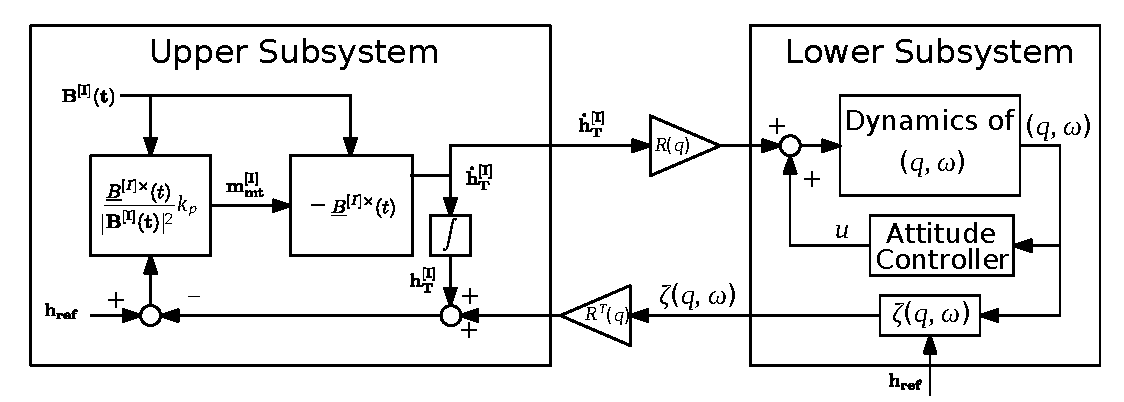
\includegraphics[page=1,width=1\textwidth]{quasiCascadeDesat.pdf}
	\end{tabular}
	\caption{Quasi cascaded desaturation control scheme \cite[Fig. 2.]{DesatTregouet}}
	\label{fig:quasiCascadeDesat}
\end{figure}

According to equation \todo{ref eq in modelling}

\begin{equation}
\underline{I}_{s}\vec{\dot{\omega}} + \underline{\omega}^\times\underline{I}_{s}\vec{\omega} = -\vec{\dot{h}}_{rw} -  \underline{\omega}^\times \vec{{h}}_{rw} + \vec{N_{mt}}  + \vec{N_{dist}} = \vec{u} 
\end{equation}

\begin{equation}
\vec{\tau_m}^{[I]} = -\frac{\underline{\tilde{b}}^\times(t)}{|\vec{\tilde{b}}(t) |^2} k_p\left(\vec{h_{rw}}^{[I]} - \underline{R}^T(\vec{q})\vec{h_{ref}} \right)
\end{equation}

\todo{make it a system of equations}

%\begin{equation}
%\dot{x}_c = 0, (\vec{q},\vec{\omega},x_c) \in C\
%\end{equation}
%
%\begin{equation}
%x_c^+ = -x_c, (\vec{q},\vec{\omega},x_c) \in D\
%\end{equation}
%
%\begin{equation}
%\vec{u} = -c x_c \epsilon -K_\omega \vec{\omega}
%\end{equation}
%
%\begin{equation}
%C:= \left\lbrace (\vec{q},\vec{\omega},x_c) \in \mathbb{S}^3 \times \mathbb{R}^3 \times \left\lbrace -1,1 \right\rbrace : x_c\eta \geq -\delta \right\rbrace 
%\end{equation}
%
%\begin{equation}
%D:= \left\lbrace (\vec{q},\vec{\omega},x_c) \in \mathbb{S}^3 \times \mathbb{R}^3 \times \left\lbrace -1,1 \right\rbrace : x_c\eta \leq -\delta \right\rbrace 
%\end{equation}

as shown in \ref{eq:finaleq}
\begin{flalign}
\vec{ ^s_i\dot q(t)}  = \dfrac{1}{2} \underline \Omega \  \vec{^s_i q(t)}
\end{flalign} 

%\[
%\begin{array}{l}
%
%\dot{x}_c = 0, (\vec{q},\vec{\omega},x_c) \in C\ \\ 
%x_c^+ = -x_c, (\vec{q},\vec{\omega},x_c) \in D\ \\ 
%\vec{u} = -c x_c \epsilon -K_\omega \vec{\omega} \\
%C:= \left\lbrace (\vec{q},\vec{\omega},x_c) \in \mathbb{S}^3 \times \mathbb{R}^3 \times \left\lbrace -1,1 \right\rbrace : x_c\eta \geq -\delta \right\rbrace  \\
%
%D:= \left\lbrace (\vec{q},\vec{\omega},x_c) \in \mathbb{S}^3 \times \mathbb{R}^3 \times \left\lbrace -1,1 \right\rbrace : x_c\eta \leq -\delta \right\rbrace 
%\end{array}
%\]

\todo{this attitude controller should be down as one of the possible attitude controllers - "Satellite angular momentum removal utilizing the earth’s magnetic field" article}

\begin{figure}[h]
	\centering
	\begin{tabular}{@{}c@{\hspace{.5cm}}c@{}}
		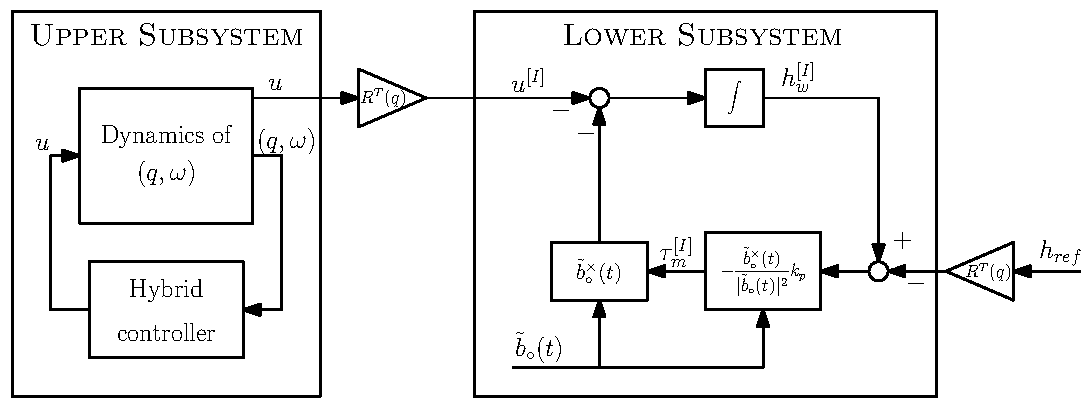
\includegraphics[page=1,width=1\textwidth]{cascadeDesat.pdf}
	\end{tabular}
	\caption{Cascaded desaturation control scheme  \cite[Fig. 4.]{DesatTregouet}}
	\label{fig:CascadeDesat}
\end{figure}

The derived equations that can be implemented in simulation:

\begin{equation}
\vec{\dot{\omega}} = \underline{I}_{s}^{-1}\left( \vec{u} -  \underline{\omega}^\times\underline{I}_{s}\vec{\omega}  \right) 
\end{equation}

\begin{equation}
\vec{\dot{h}}_{rw} =  -  \underline{\omega}^\times \vec{{h}}_{rw} + \vec{N_{mt}}  + \vec{N_{dist}} - \vec{u} 
\end{equation}

\todo{body-fixed frame
	Static input allocation
	global asymptotic stability}

\cite{DesatYang}